\section[塞曼效应]{塞曼效应} \label{sec:07.05} % 
% \makebox[5em][s]{} % 短题目拉间距

早在19世纪末就已经发现磁场能够影响原子光谱.1896年塞曼发现,如将光源放在磁场中,则每一条光谱线均分裂成一组相邻的线.这种现象称为塞曼效应.

显然, 谱线分裂的根源是能级分裂.以单价原子为例,其光谱产生于价电子的能级跃迁未加磁场前,价电子的能量算符可以写成(参看$\S$\ref{sec:07.03})
\begin{empheq}{equation}\label{eq75.1}
	H_{0}=\frac{\boldsymbol{p}^{2}}{2m_{e}}+V(r)+\xi(r)\boldsymbol{S}\cdot\boldsymbol{L}
\end{empheq}
最后一项是自旋轨道耦合能加上磁场后,价电子又获得一项磁作用势,以磁场方向为$z$轴,磁作用势为
\begin{empheq}{equation}\label{eq75.2}
	H^{\prime}=-\boldsymbol{B}\cdot(\boldsymbol{\mu_{L}}+\boldsymbol{\mu_{S}})=\frac{eB}{2m_{e}c}(L_{z}+2S_{z})
\end{empheq}
[参看\eqref{eq74.25}式,略去很小的逆磁性项($B^{2}$项).]价电子的总能量算符变成
\eqshort
\begin{empheq}{equation}\label{eq75.3}
	H=H_{0}+H^{\prime}
\end{empheq}\eqnormal
由$H^{\prime}$造成的能级分裂,视磁场的强弱而有所不同.

{\heiti 1. 强磁场,简单塞曼效应}

如磁场很强(至少要几十万高斯),以致\eqref{eq75.1}式中自旋轨道耦合能可以忽略不计,这时价电子的能量算符为
\begin{empheq}{equation}\label{eq75.4}
	H=\frac{\boldsymbol{p}^{2}}{2m_{e}}+V(r)+\frac{eB}{2m_{e}c}(L_{z}+2S_{z})
\end{empheq}
其中第三项为磁作用势.这时$H,H_{0},\boldsymbol{L}^{2},L_{z},S_{z}$是互相对易的守恒量.如以$E_{nl}^{(0)}$表示$H_{0}=(\hat{T}+V)$的本征值(未加磁场时的价电子能级),$\varPsi_{nlm}=R_{nl}(r)Y_{lm}(\theta\varphi)$表示$(H_{0},\boldsymbol{L}^{2},L_{z})$共同本征函数,则$(H,\boldsymbol{L}^{2},L_{z},S_{z})$的共同本征函数显然是
\begin{empheq}{equation}\label{eq75.5}
	\varPsi_{nlmm_{s}}=\varPsi_{nlm}\chi_{1/2},\quad \varPsi_{nlm}\chi_{-1/2}
\end{empheq}
前者$S_{z}=\frac{\hbar}{2}\bigg(m_{s}=\frac{1}{2}\bigg)$,后者$S_{z}=-\frac{\hbar}{2}\bigg(m_{s}=-\frac{1}{2}\bigg)$.能级可以记成$E=E_{nlmm_{s}}$,显然
\begin{empheq}{align}\label{eq75.6}
	E_{nlmm_{s}}&=E_{nl}^{(0)}+B\mu_{B}(m+2m_{s})	\nonumber\\
	&=E_{nl}^{(0)}+\begin{dcases}
		(m+1)B\mu_{B},\quad m_{s}=\frac{1}{2}	\\
		(m-1)B\mu_{B},\quad m_{s}=-\frac{1}{2}
	\end{dcases}
\end{empheq}
$\bigg(\mu_{B}$为玻尔磁子$\bigg)$上式表明,能级$E_{nl}^{(0)}$在磁场中分裂成一组等距离的能级,能级间距为$B\mu_{B}$.由能级跃迁产生的光谱线也有分裂现象,由于跃迁选择定则:
\begin{empheq}{equation}\label{eq75.7}
	\Delta l=\pm1,\quad \Delta m=0,\pm1,\quad \Delta m_{s}=0
\end{empheq}
的限制,每条谱线在磁场中分裂成三条等距离的谱线.能级和谱线的分裂如图\ref{fig.7-2}所示.

\begin{figure}[!h]
	\centering
	\small
	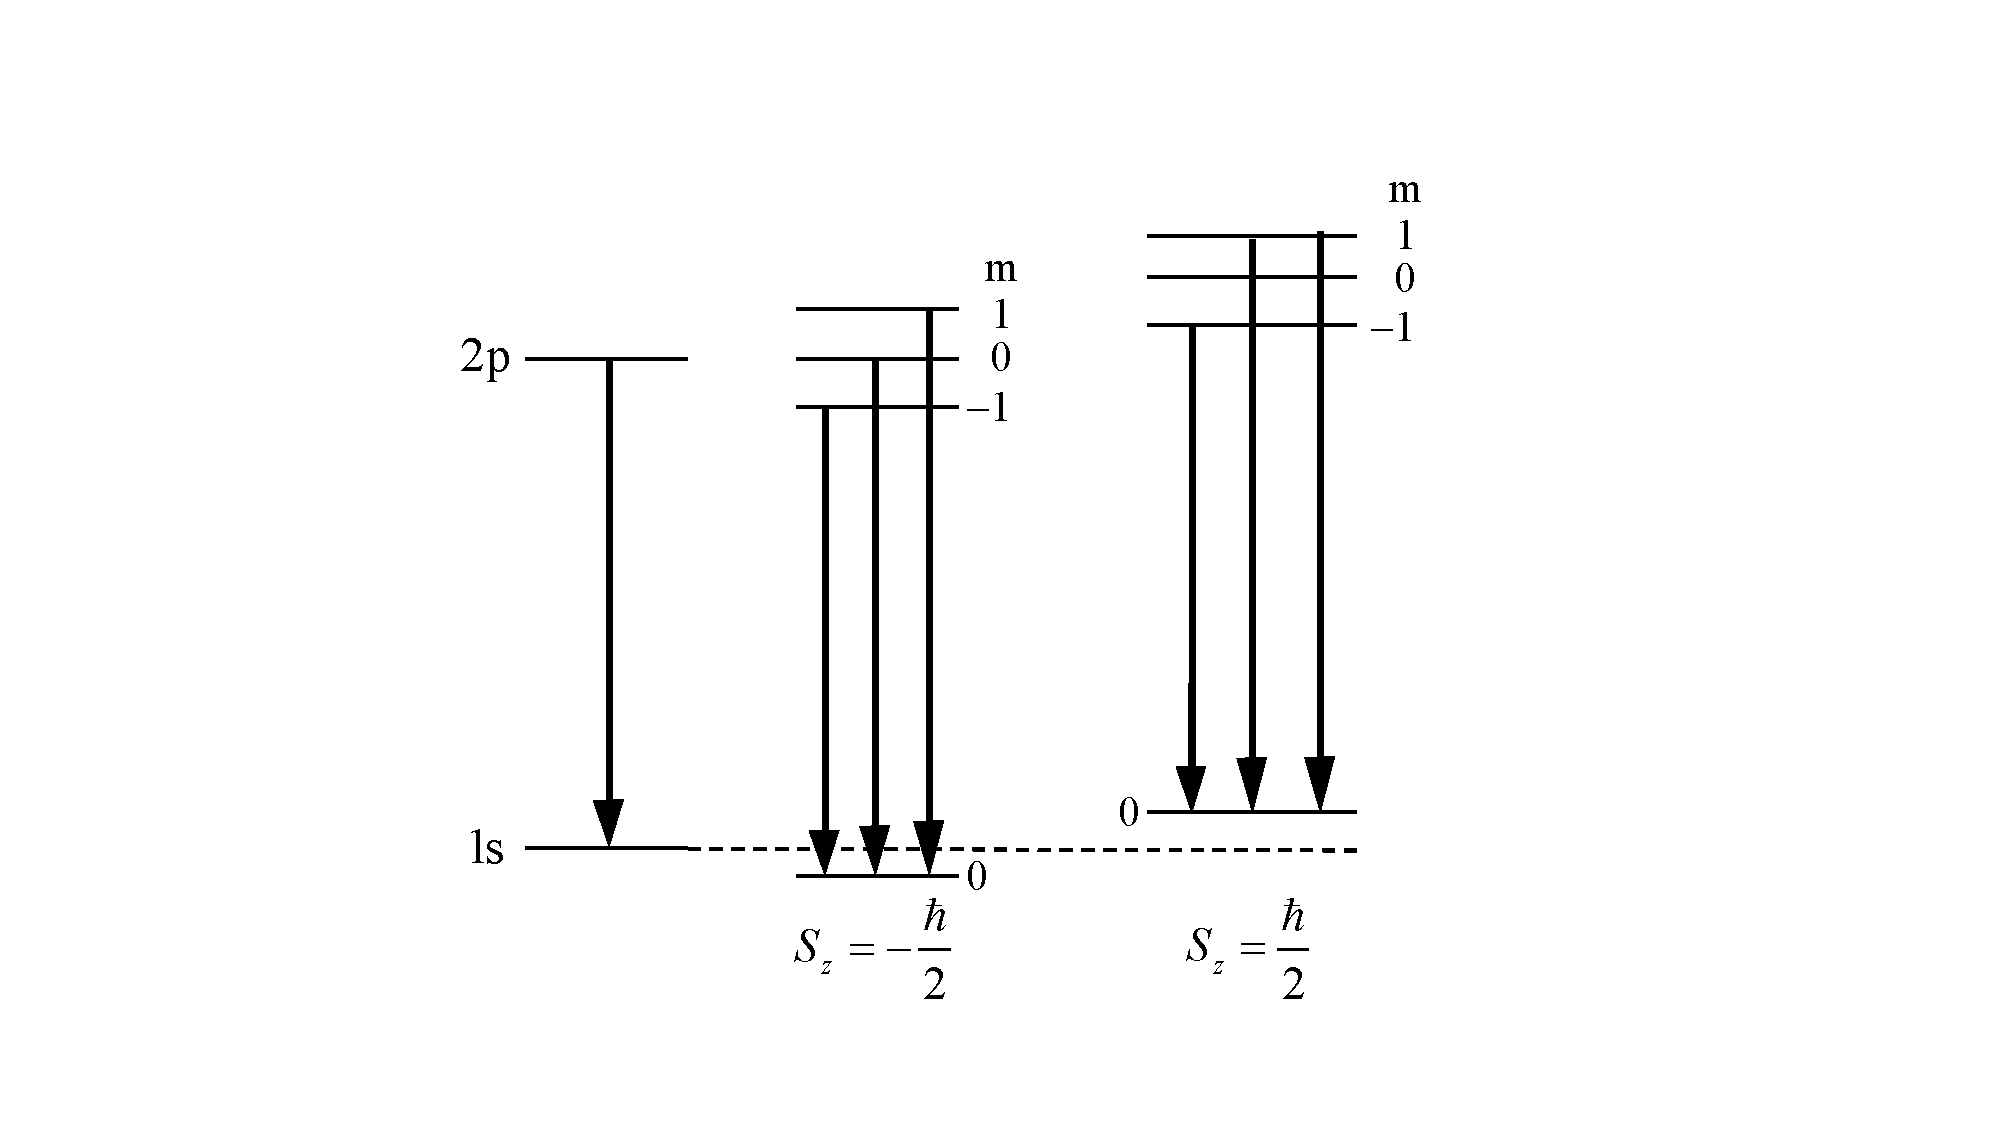
\includegraphics[width=5cm,clip]{QM file/figure/7-2}
	\caption{}\label{fig.7-2}
\end{figure}

图\ref{fig.7-2}画出了能级$E_{21}^{(0)}$,$E_{10}^{(0)}$在强磁场中的分裂示意图,以及符合选择定则的能级跃迁.由于跃迁前后自旋量子数$m_{s}$不变,图中两组跃迁产生的光谱相同,均包含三条谱线.相邻谱线的频率差为
\begin{empheq}{equation}\label{eq75.8}
	\Delta\omega=\frac{B\mu_{B}}{\hbar}=\frac{eB}{2m_{e}c}
\end{empheq}
刚好等于经典拉摩频率.这种现象,称为简单塞曼效应\footnote{
单价原子光谱在强磁场中的分裂现象,严格说应称为帕邢-巴克(Paschen-Back)效应.纯粹的简单塞曼效应只产生于价电子为偶数,总自旋角动量$S=0$的情况下,这时自旋轨道耦合能为0.磁作用势
\begin{empheq}{equation*}
	H^{\prime}=-\boldsymbol{B}\cdot\mu_{L}=\frac{eB}{2m_{e}c}L_{z}
\end{empheq}
($\boldsymbol{L}$为总轨道角动量)能级变化为$H^{\prime}=mB\mu_{B}(L_{z}=m\hbar)$,能级$E_{nl}^{(0)}$分裂成$(2L+1)$条等距离能级,间距$\Delta E=B\mu_{B}$.由于跃迁选择定则\eqref{eq75.7}式的制约,光谱线仍分裂为三条等距离的谱线,$\Delta\omega$仍由\eqref{eq75.8}式表示.这种效应只需要弱磁场就能产生,而且可以给以经典电动力学解释,所以曾称为正常塞曼效应.其实下面要讲的复杂塞曼效应才是塞曼效应的一般表现形式,由于它无法用经典物理理论来解释,曾被称为“反常”的.}由于$\Delta\omega$与$\hbar$无关,历史上曾根据经典电动力学的拉摩进动模型给出了很好的定量解释.

{\heiti 2. 弱磁场,复杂塞曼效应}

在弱磁场中,单价原子受到的磁作用势小于自旋轨道耦合能,应将\eqref{eq75.3}式中$H^{\prime}$作为微扰.取$(H_{0},\boldsymbol{L}^{2},\boldsymbol{J}^{2},J_{z})$共同本征函数作为零级近似波函数,记为
\begin{empheq}{equation}\label{eq75.9}
	\Psi_{nljm_{j}}^{(0)}=R_{nl}(r)\varPsi_{ljm_{j}}(\theta,\varphi,S_{z})
\end{empheq}
其中$\varPsi_{ljm_{j}}$表示$(\boldsymbol{L}^{2},\boldsymbol{J}^{2},J_{z})$共同本征函数(见$\S$\ref{sec:07.02}).$H_{0}$由\eqref{eq75.1}式表示,其中包含了自旋轨道耦合能.$H_{0}$的本征值即未加磁场时的价电子能级,和量子数$nlj$有关,但和$m_{j}$无关,(见$\S$\ref{sec:07.03})可以记为$E_{nlj}^{(0)}$,能级简并度$(2j+1)$.给定$n,l$后,$j=l\pm\frac{1}{2}$对应于两个能级,就是能级的精细结构(见$\S$\ref{sec:07.03}).

按照简并态微扰论计算磁作用势$H^{\prime}$造成的能级变化(一级修正).由于$H^{\prime}$与$J_{z}$对易,因此$H^{\prime}$的非对角矩阵元全部等于0,能级的一级修正等于$H^{\prime}$对\eqref{eq75.9}式的平均值,即
\eqlong
\begin{empheq}{align}\label{eq75.10}
	E_{nljm_{j}}^{(1)} &=\int\Psi_{nljm_{j}}^{(0)+}\hat{H}\Psi_{nljm_{j}}^{(0)}d\tau	\nonumber\\
	&=\frac{eB}{2m_{e}c}(\overline{J_{z}}+\overline{S_{z}})=\frac{eB}{2m_{e}c}\bigg(m_{j}\hbar+\frac{\hbar}{2}\overline{\sigma_{z}}\bigg)
\end{empheq}\eqnormal
其中$\overline{\sigma_{z}}$已在\eqref{eq72.23}式、\eqref{eq72.24}式算出,为
\begin{empheq}{align}\label{eq75.11}
	\overline{\sigma_{z}}=
	\begin{dcases}
		\quad\frac{m_{j}}{j},\qquad j=l+\frac{1}{2}	\\
		-\frac{m_{j}}{j+1},\quad j=l-\frac{1}{2}
	\end{dcases}
\end{empheq}
代入\eqref{eq75.10}式, 即得
\begin{empheq}{equation}\label{eq75.12}
	E_{nljm_{j}}^{(1)}=B\mu_{B}m_{j}g
\end{empheq}
其中$g$为朗德$g$因子,即
\eqlong
\begin{empheq}{align}\label{eq75.13}
	g &=1+\frac{\langle\sigma_{z}\rangle}{2m_{j}}=1+\frac{\langle S_{z}\rangle}{\langle J_{z}\rangle}	\\
	&=\begin{dcases}
		1+\frac{1}{2j},\qquad\quad	j=l+\frac{1}{2}	\\
		1-\frac{1}{2j+2},\quad j=l-\frac{1}{2}	
	\end{dcases}	\nonumber \tag{$7.5.13^{\prime}$}
\end{empheq}\eqnormal
这样, 由\eqref{eq75.12}式、\eqref{eq75.13}式可知,能级$E_{nlj}^{(0)}$在弱磁场中分裂成$(2j+1)$个等距离能级,相应于$m_{j}$的$(2j+1)$种取值
\begin{empheq}{equation}\label{eq75.14}
	m_{j}=j,j-1,\cdots,(-j)
\end{empheq}
能级间距为$B\mu_{B}g$.(在简单塞曼效应中,能级分裂间距为$B\mu_{B}$)因此,对光谱进行实验分析浏定,可以推断出能级的$g$和$j$值(由此也就知道$l$值),这样就获得了有关原子结构的重要信息.

能级跃迁的选择定则是
\begin{empheq}{equation}\label{eq75.15}
	\Delta l=\pm1,\quad \Delta j=0,\pm1,\quad \Delta m_{j}=0,\pm1
\end{empheq}
图\ref{fig.7-3}画出了钠(\ce{Na})的$D_{1}$和$D_{2}$线的分裂示意图.能级和谱线的分裂均比简单塞曼效应复杂,故称复杂塞曼效应.发现这现象的当时,无法对此作出理论解释,故又称反常塞曼效应.直到1925年乌仑贝克(Uhlenbeck)与古兹米特(Goudsmit)提出电子自旋假设,这个“反常”现象才得到解释.

\begin{figure}[!h]
	\centering
	\small
	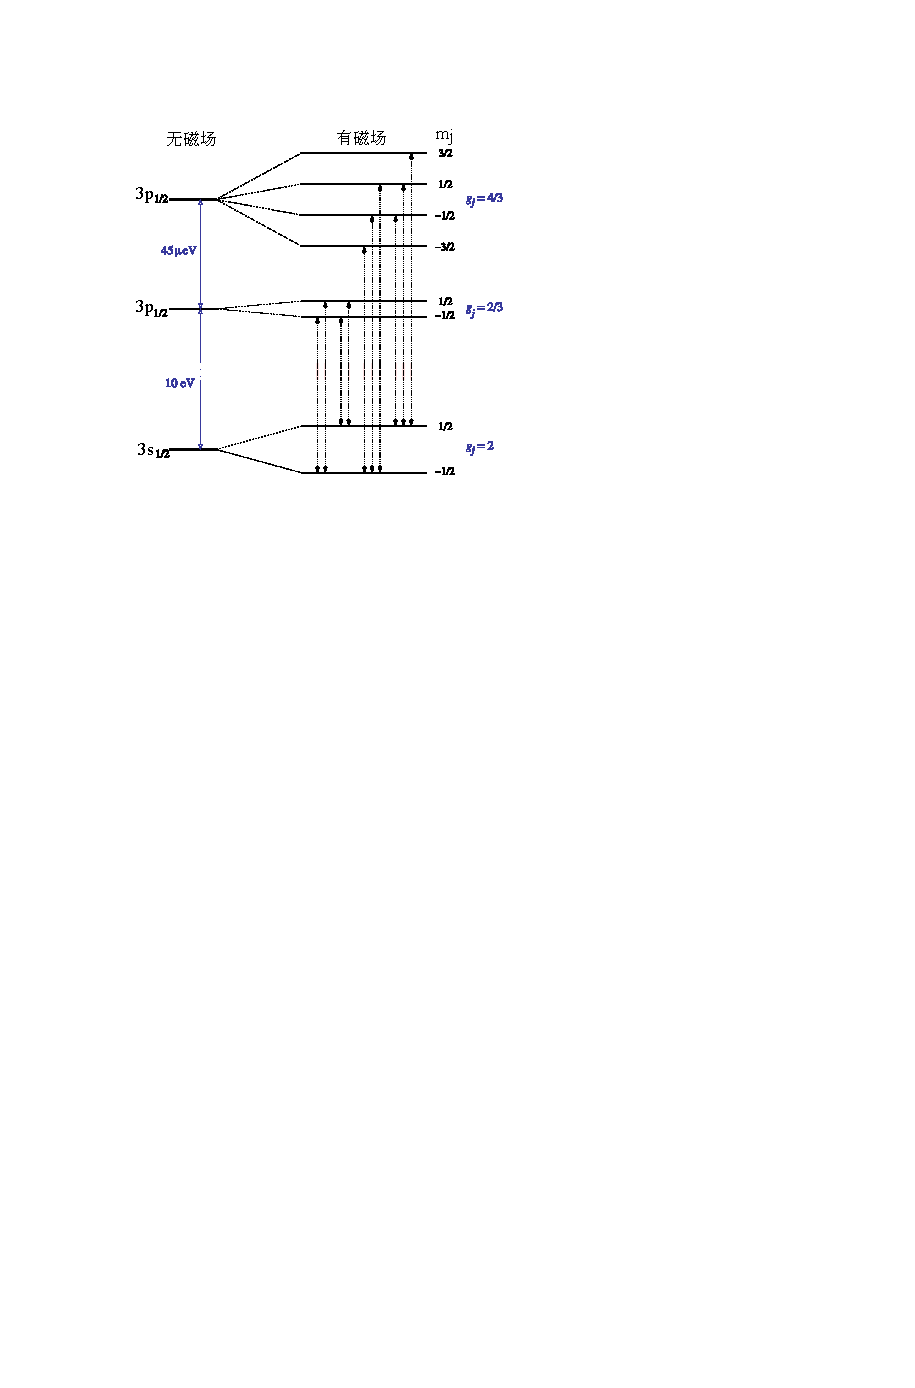
\includegraphics[width=5cm,clip]{QM file/figure/7-3}
	\caption{}\label{fig.7-3}
\end{figure}


\example 证明朗德$g$因子也可以表示成
\eqlong
\begin{empheq}{equation}\label{eq75.16}
	g=1+\frac{j(j+1)+s(s+1)-l(l+1)}{2j(j+1)}\quad \bigg(s=\frac{1}{2}\bigg)
\end{empheq}\eqnormal

\solution 由\eqref{eq72.27}式,可得(以下各式中,$\boldsymbol{\sigma}\cdot\boldsymbol{L}$均指其本征值.$\hbar$均略去不写)
\eqshort
\begin{empheq}{equation}\label{eq75.17}
	\overline{S_{z}}=\frac{m_{j}}{1+2\boldsymbol{\sigma}\cdot\boldsymbol{L}}
\end{empheq}\eqnormal
而\eqref{eq72.5}式取本征值,有
\begin{empheq}{equation}\label{eq75.18}
	j(j+1)=l(l+1)+\frac{3}{4}+\boldsymbol{\sigma}\cdot\boldsymbol{L}
\end{empheq}
利用\eqref{eq72.11}式消去$l(l+1)$,成为
\begin{empheq}{equation}\label{eq75.19}
	\begin{aligned}
		j(j+1)&=(\boldsymbol{\sigma}\cdot\boldsymbol{L})^{2}+2\boldsymbol{\sigma}\cdot\boldsymbol{L}+\frac{3}{4}	\\
		&=\bigg(\boldsymbol{\sigma}\cdot\boldsymbol{L}+\frac{1}{2}\bigg)\bigg(\boldsymbol{\sigma}\cdot\boldsymbol{L}+\frac{3}{2}\bigg)
	\end{aligned}
\end{empheq}
利用此式,可将\eqref{eq75.17}式变成
\begin{empheq}{align}\label{eq75.20}
	\frac{\overline{S_{z}}}{m_{j}} &=\frac{\boldsymbol{\sigma}\cdot\boldsymbol{L}+\frac{3}{2}}{2j(j+1)},\text{再\eqref{eq75.18}利用式,}	\nonumber\\
	&=\frac{j(j+1)+\frac{3}{4}-l(l+1)}{2j(j+1)}
\end{empheq}
再代入\eqref{eq75.13}式,即得
\eqlong
\begin{empheq}{equation*}
	g=1+\frac{\overline{S_{z}}}{m_{j}\hbar}=1+\frac{j(j+1)+\frac{3}{4}-l(l+1)}{2j(j+1)}
\end{empheq}\eqnormal
此即\eqref{eq75.16}式.